\documentclass[11pt, aspectratio=169, table]{beamer}

% --- Tema y configuración general ---
\usetheme{Madrid}
\usecolortheme{default}

% --- Paquetes ---
\usepackage[utf8]{inputenc}
\usepackage[T1]{fontenc}
\usepackage[spanish]{babel}
\usepackage{graphicx}
\usepackage{booktabs}
\usepackage{amsmath}
\usepackage{amssymb}
% (beamer ya carga xcolor; la opción table viene de la clase)
\usepackage{array}
\usepackage{threeparttable}
\usepackage[backend=biber,style=authoryear]{biblatex}
\addbibresource{referencias.bib}

\def\sym#1{\ifmmode^{#1}\else\(^{#1}\)\fi}

% --- Color de acento ---
\definecolor{azul}{RGB}{0, 102, 204} % Un azul bonito y legible
\setbeamercolor{structure}{fg=azul}

% --- Información del documento ---
\title[Entrega y satisfacción]{Tiempo de entrega y satisfacción del cliente en e-commerce}
\subtitle{Una aplicación de regresión lineal múltiple y regresión logística}
\author[Aranguren]{Valeria Aranguren\\[0.2em]
    {\small Analítica de los Negocios, Pontificia Universidad Javeriana}}
\date{Noviembre de 2026}

\begin{document}

%=================================================================
% 1. PORTADA
%=================================================================
\begin{frame}
    \titlepage
\end{frame}

%=================================================================
% 2. MOTIVACIÓN Y PREGUNTA
%=================================================================
\section{Motivación}
\begin{frame}{Motivación y pregunta}
    \begin{itemize}
        \setlength\itemsep{0.55em}
        \item En e-commerce, la entrega es uno de los pocos contactos tangibles con el cliente.
        \item La literatura sugiere que lo que importa no es cuánto se demora el envío, sino si cumple lo prometido.
        \item \textbf{Pregunta:} ¿cómo se relaciona la diferencia entre la entrega real y la prometida con la satisfacción del cliente?
        \item Dos mediciones de satisfacción: calificación (1-5 estrellas) y sentimiento de la reseña (positiva o no).
    \end{itemize}

    \vspace{0.3em}
    \begin{alertblock}{Importante}
        Los datos son observacionales: los resultados son \textbf{asociaciones}, no efectos causales.
    \end{alertblock}
\end{frame}

%=================================================================
% 3. MARCO TEÓRICO
%=================================================================
\section{Marco teórico}
\begin{frame}{Marco teórico}
    \begin{itemize}
        \setlength\itemsep{0.5em}
        \item \textcite{akturk2022}: la desviación entre entrega real y prometida explica las calificaciones; tarde castiga, temprano premia (efectos curvilíneos).
        \item \textcite{nozari2026}: con millones de compras, las entregas tardías reducen las calificaciones de los productos.
        \item \textcite{ravula2023}: el castigo por llegar tarde es mayor que el premio por llegar temprano (asimetría).
        \item \textcite{deshpande2023}: el desempeño logístico se conecta con calificaciones y con ventas posteriores.
        \item \textcite{rao2011} y \textcite{harter2025}: las fallas de entrega reducen la recompra.
    \end{itemize}
\end{frame}

%=================================================================
% 4. DATOS
%=================================================================
\section{Datos}
\begin{frame}{Datos}
    \begin{itemize}
        \setlength\itemsep{0.55em}
        \item 138.116 pedidos de una plataforma de e-commerce; muestra de análisis: \textbf{113.559 pedidos entregados}.
        \item 24.557 pedidos cancelados o pendientes se excluyen (no tienen calificación ni tiempos).
        \item \textbf{Variable central:} diferencia de entrega = días reales $-$ días prometidos.
        \item Controles: edad, género, tipo de cliente y método de envío.
    \end{itemize}

    \vspace{0.3em}
    \begin{center}
        \renewcommand{\arraystretch}{1.15}
        \small
        \begin{tabular}{lccc}
            \toprule
            \textbf{Variable} & \textbf{Media} & \textbf{Desv. est.} & \textbf{Rango} \\
            \midrule
            Calificación (1-5) & 3,68 & 0,48 & 1,6 a 5 \\
            Días de entrega reales & 4,56 & 2,81 & 0 a 14 \\
            Días de entrega prometidos & 4,30 & 2,59 & 0 a 10 \\
            \rowcolor{green!18}
            \textbf{Diferencia de entrega} & \textbf{0,26} & \textbf{1,12} & \textbf{-2 a 4} \\
            Edad del cliente & 45,9 & 16,5 & 18 a 74 \\
            \bottomrule
        \end{tabular}
    \end{center}
\end{frame}

\begin{frame}{Datos: hechos exploratorios}
    \begin{columns}[T]
        \begin{column}{0.5\textwidth}
            \begin{itemize}
                \setlength\itemsep{0.5em}
                \item 63,3\% de los pedidos llega exactamente en la fecha prometida.
                \item Retrasos de hasta 4 días; entregas tempranas de hasta 2.
                \item De las reseñas: 68,8\% positivas, 30,5\% neutrales, 0,7\% negativas.
                \item Como las negativas son tan pocas, \textbf{neutral se agrupa con negativa} (decisión documentada).
            \end{itemize}
        \end{column}
        \begin{column}{0.48\textwidth}
            \centering
            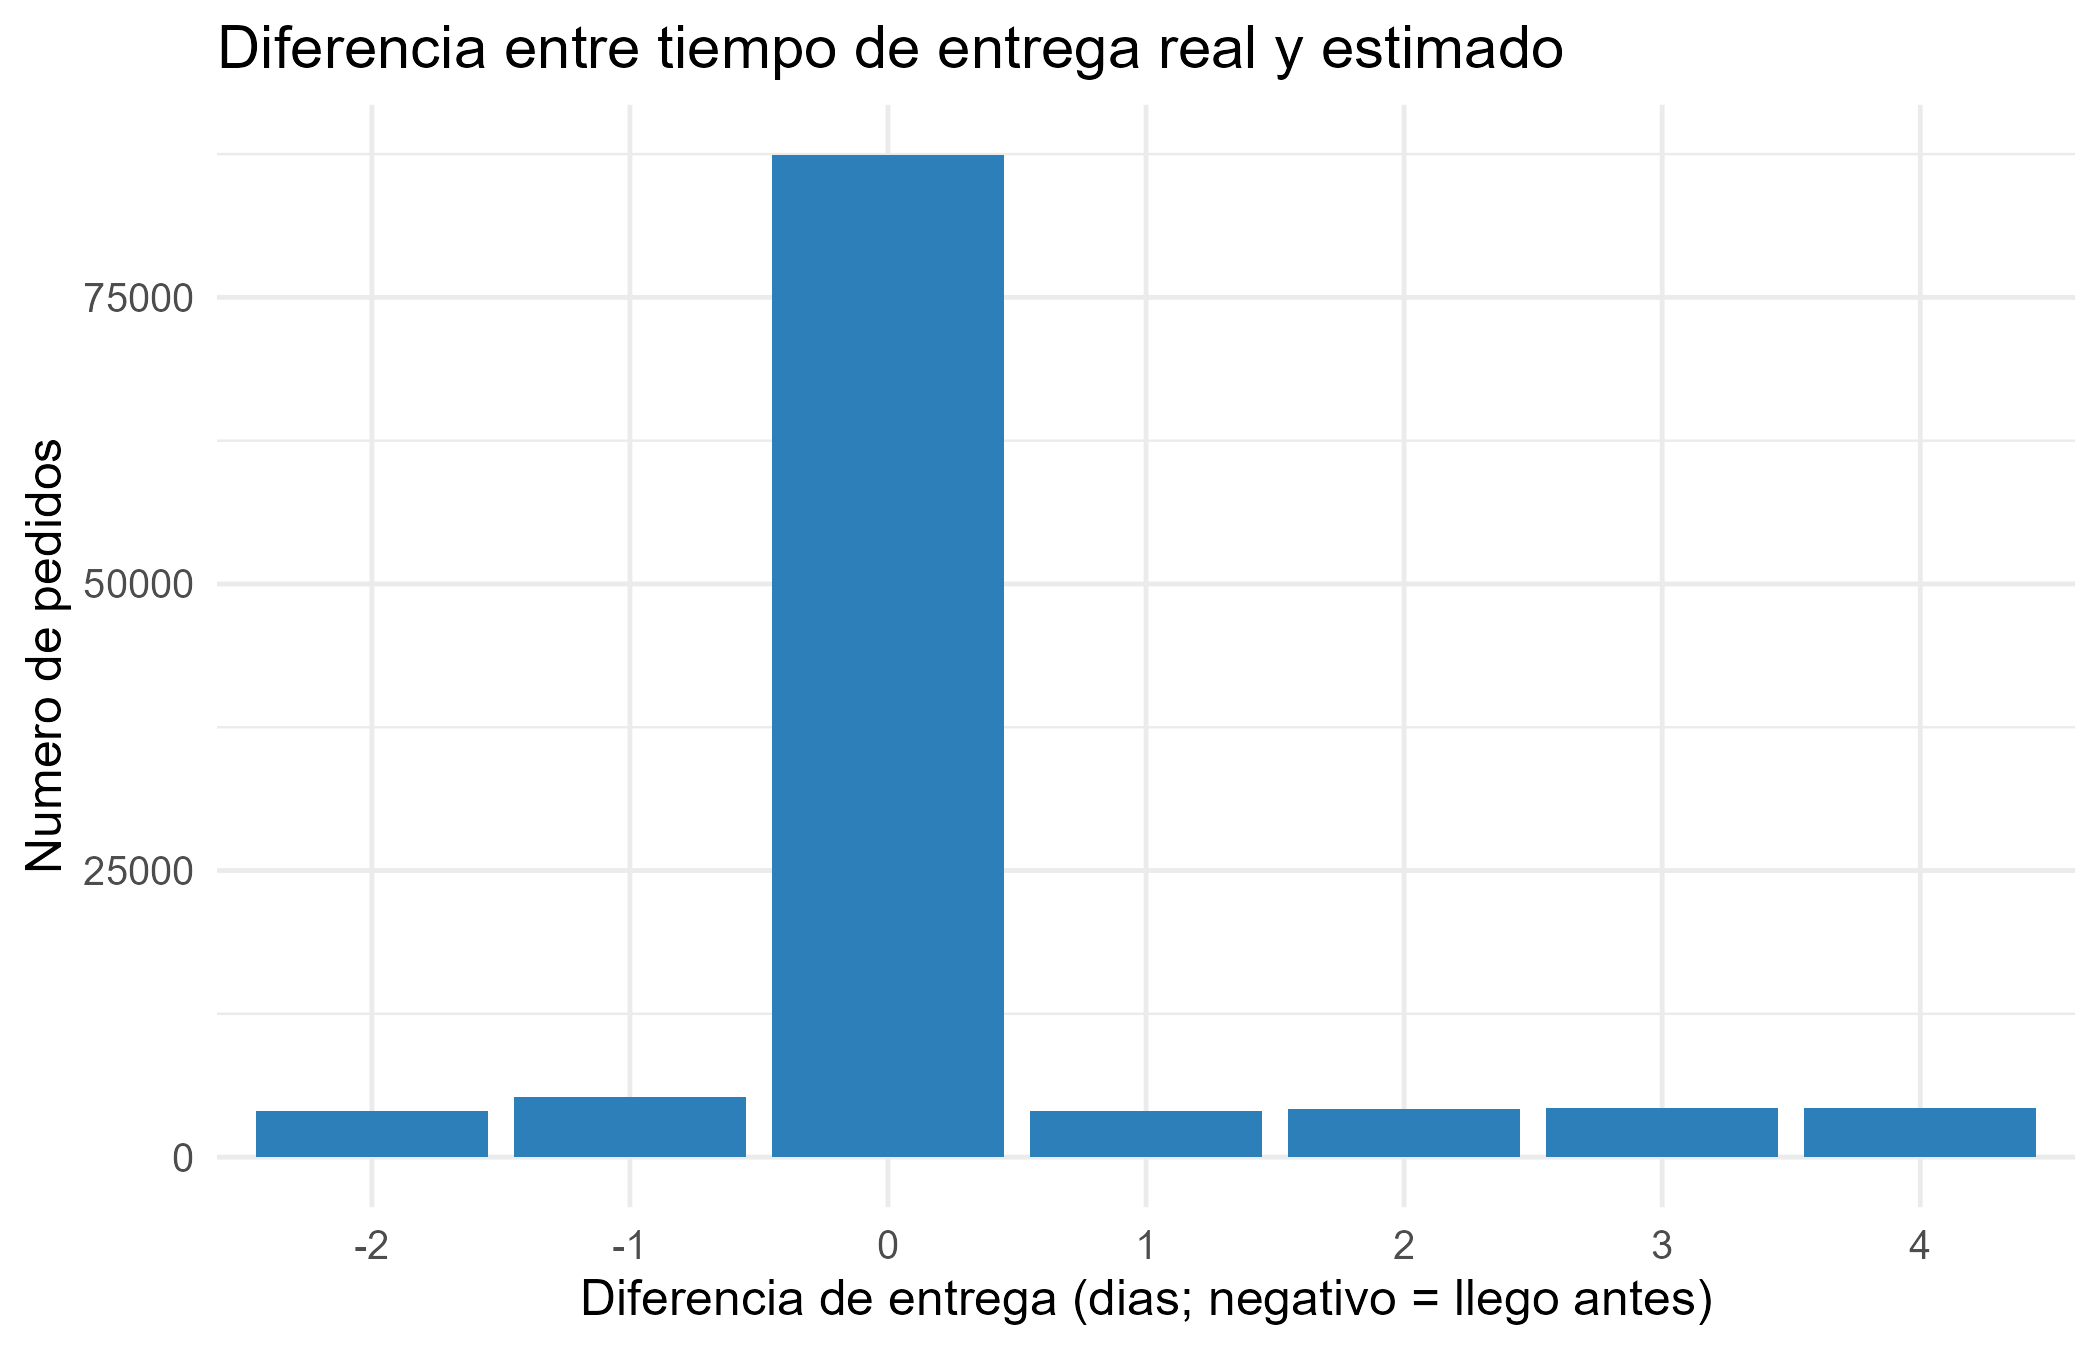
\includegraphics[width=\textwidth]{salidas/figuras/fig_03_barras_diferencia.png}\\
            {\small Distribución de la diferencia de entrega.}
        \end{column}
    \end{columns}
\end{frame}

\begin{frame}{El patrón clave en los datos}
    \centering
    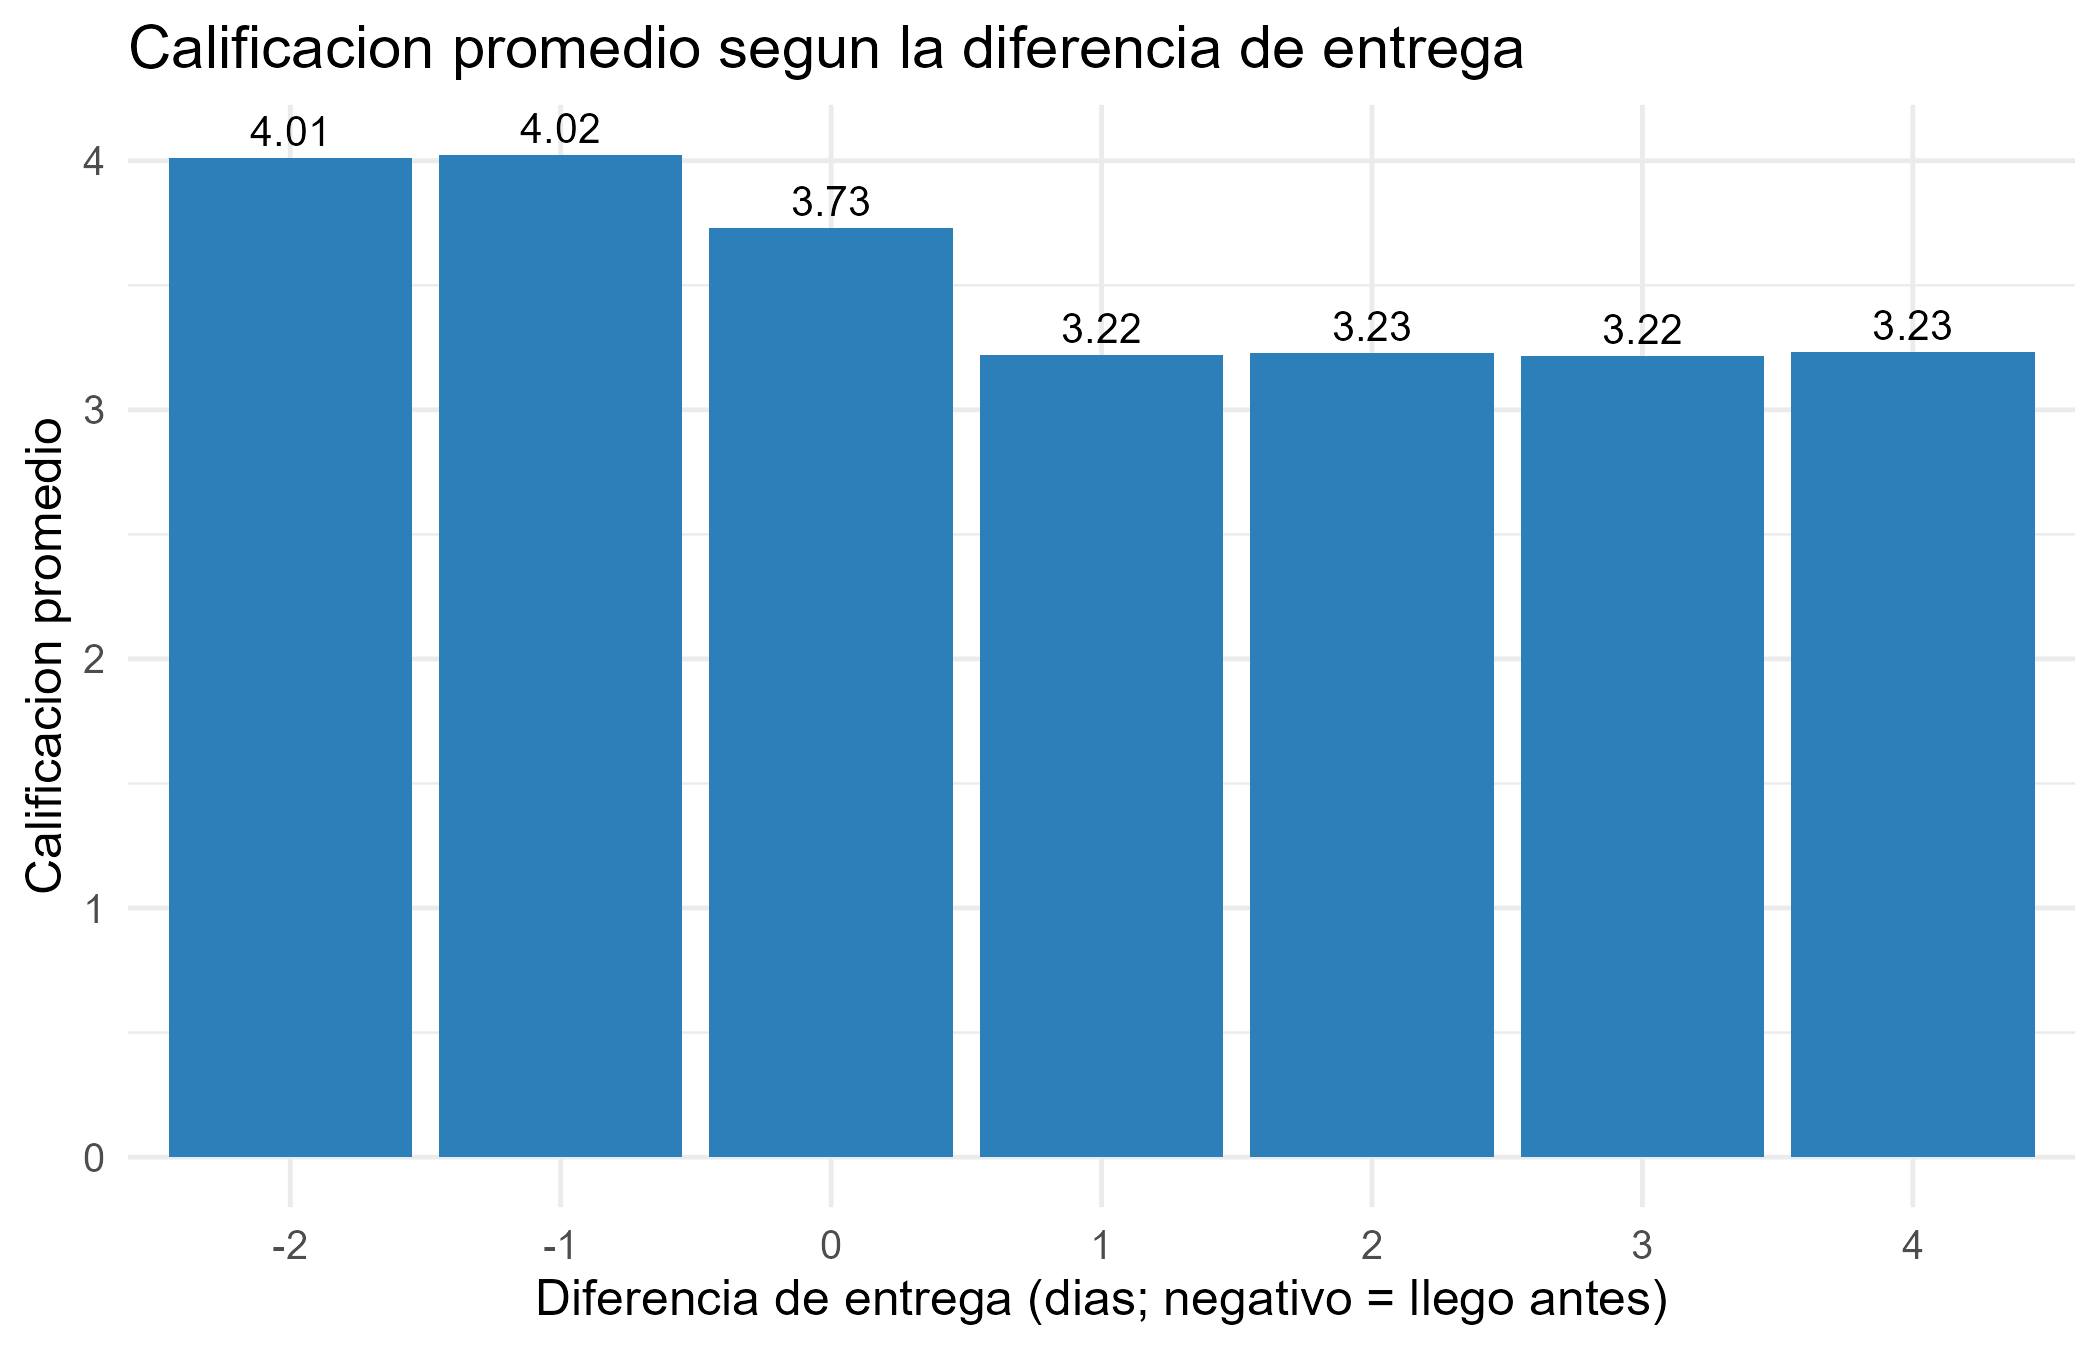
\includegraphics[width=0.58\textwidth]{salidas/figuras/fig_04_rating_por_diferencia.png}

    \vspace{0.3em}
    {\small \textit{La calificación promedio cae casi de forma monótona con el retraso frente a lo prometido.}}
\end{frame}

%=================================================================
% 5. METODOLOGÍA
%=================================================================
\section{Metodología}
\begin{frame}{Metodología}
    \begin{columns}[T]
        \begin{column}{0.48\textwidth}
            \textbf{1. Regresión lineal múltiple (MCO)}
            \[
                \text{rating}_i = \beta_0 + \beta_1\,\text{dif. entrega}_i + \mathbf{\gamma}'\mathbf{X}_i + \varepsilon_i
            \]
            $\beta_1$: cambio en estrellas por cada día de retraso.
        \end{column}
        \begin{column}{0.48\textwidth}
            \textbf{2. Modelo logit}
            \[
                \Pr(\text{positiva}_i) = \Lambda\!\left(\beta_0 + \beta_1\,\text{dif. entrega}_i + \mathbf{\gamma}'\mathbf{X}_i\right)
            \]
            Se reportan \textit{odds ratios}: $<1$ = menor probabilidad de reseña positiva.
        \end{column}
    \end{columns}

    \vspace{0.5em}
    \begin{block}{Robustez y límites}
        Se reestima todo con \texttt{atrasado} (1 = llegó tarde). Límites: calificación acotada entre 1 y 5 tratada como continua; interpretación de asociación, no causal.
    \end{block}
\end{frame}

%=================================================================
% 6. RESULTADOS
%=================================================================
\section{Resultados}
\begin{frame}{Resultados: regresión lineal múltiple}
    \begin{center}
        \renewcommand{\arraystretch}{1.15}
        \small
        \begin{tabular}{lcc}
            \toprule
            \textbf{Variable} & \textbf{Coeficiente} & \textbf{(Err. est.)} \\
            \midrule
            \rowcolor{green!18}
            \textbf{Diferencia de entrega (días)} & \textbf{-0,167\sym{***}} & (0,001) \\
            Días de entrega prometidos & -0,002 & (0,001) \\
            Edad, género, tipo de cliente, envío & \multicolumn{2}{c}{no significativos} \\
            \midrule
            $R^2$ & \multicolumn{2}{c}{0,149 \quad ($n = 113559$)} \\
            \bottomrule
        \end{tabular}
    \end{center}
    \vspace{0.3em}
    \begin{itemize}
        \item Cada día de retraso frente a la promesa se asocia con \textbf{0,167 estrellas menos}.
        \item La duración prometida del envío \textbf{no} se asocia con la calificación.
    \end{itemize}
\end{frame}

\begin{frame}{Resultados: modelo logit}
    \begin{center}
        \renewcommand{\arraystretch}{1.15}
        \small
        \begin{tabular}{lcc}
            \toprule
            \textbf{Variable} & \textbf{Odds ratio} & \textbf{IC 95\%} \\
            \midrule
            \rowcolor{green!18}
            \textbf{Diferencia de entrega (días)} & \textbf{0,528} & (0,521 - 0,535) \\
            Días de entrega prometidos & 0,995 & (0,984 - 1,005) \\
            Controles & \multicolumn{2}{c}{no significativos} \\
            \midrule
            Aciertos (corte 0,5) & \multicolumn{2}{c}{73,2\%} \\
            \bottomrule
        \end{tabular}
    \end{center}
    \vspace{0.3em}
    \begin{itemize}
        \item Cada día de retraso reduce en cerca del \textbf{47\%} las probabilidades de una reseña positiva.
    \end{itemize}
\end{frame}

\begin{frame}{Robustez: llegar tarde como variable binaria}
    \begin{center}
        \renewcommand{\arraystretch}{1.15}
        \small
        \begin{tabular}{lcc}
            \toprule
            & \textbf{MCO (calificación)} & \textbf{Logit (odds ratio)} \\
            \midrule
            \rowcolor{green!18}
            \textbf{Atrasado (sí/no)} & \textbf{-0,531\sym{***}} & \textbf{0,143} \\
            \bottomrule
        \end{tabular}
    \end{center}
    \vspace{0.3em}
    \begin{itemize}
        \setlength\itemsep{0.5em}
        \item Llegar tarde: \textbf{0,53 estrellas menos} en promedio.
        \item Llegar tarde: probabilidades de reseña positiva \textbf{86\% menores}.
        \item Lo que pesa es \textbf{incumplir la promesa}, coherente con \textcite{ravula2023} y \textcite{nozari2026}.
    \end{itemize}
\end{frame}

%=================================================================
% 7. CONCLUSIONES
%=================================================================
\section{Conclusiones}
\begin{frame}{Conclusiones}
    \begin{enumerate}
        \setlength\itemsep{0.55em}
        \item El cumplimiento de la promesa de entrega se asocia fuertemente con la satisfacción; la duración prometida, no.
        \item Cada día de retraso: -0,167 estrellas y -47\% en las probabilidades de reseña positiva; llegar tarde: -86\%.
        \item Implicación gerencial: más que acortar tiempos, fijar \textbf{promesas realistas y cumplirlas}.
        \item Límites: asociación y no causalidad; calificación acotada tratada como continua. Extensión natural: modelo ordenado.
    \end{enumerate}
\end{frame}

%=================================================================
% 8. REFERENCIAS
%=================================================================
\section{Referencias}
\begin{frame}[allowframebreaks]{Referencias}
    \printbibliography
\end{frame}

\end{document}
